\pagebreak
\subsection{Convergences and Analysis of Baseline Mesh}
%[15\%] Run your code on the baseline mesh at $\alpha = 1\degree$ , starting with a uniform freestream state at this $\alpha$. Perform the following post-processing: Plot the convergence of the given residual $L_1$ norm versus time step iterations, Plot the convergence of the ATPR output versus time step iterations, For the converged solution, make two field plots: one of the Mach number, and one of the total pressure.

After implementing my finite-volume code I will perform several convergence studies and look to the results of my solver to determine the accuracy of my implementation. In this section I will perform an $L_1$ residual norm, look at the accuracy of the solver from the results of the ATPR over time iterations, and then finally analyze the total pressure field, as well as the Mach field.

\subsubsection{$L_1$ Norm Convergence}
\begin{figure}[h]
    \centering
    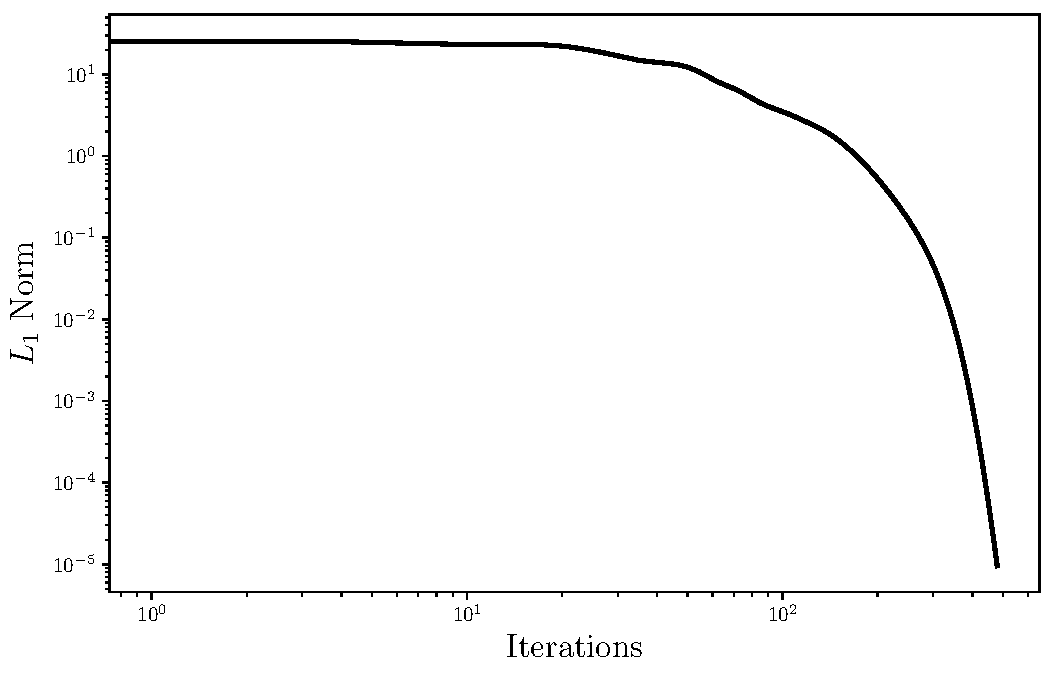
\includegraphics[width = 0.9\linewidth]{rep/q3/l1_err.pdf}
    \caption[$L_1$ Norm Convergence for Baseline Mesh]{$L_1$ norm convergence versus time step iterations.}
    \label{fig:l1_mesh0}
\end{figure}

Shown above in Figure \ref{fig:l1_mesh0}, is the convergence of $L_1$ norm as my code progresses through time-step iterations. As shown, and verified above this method will converge to an approximate answer in which the $L_1$ error is less than $10^{-5}$ to deem an accurate answer. The convergence rate is not given, since this method is conducting local-time step iterations which would not return a physical answer.

\pagebreak
\subsubsection{ATPR Output}
\begin{figure}[h]
    \centering
    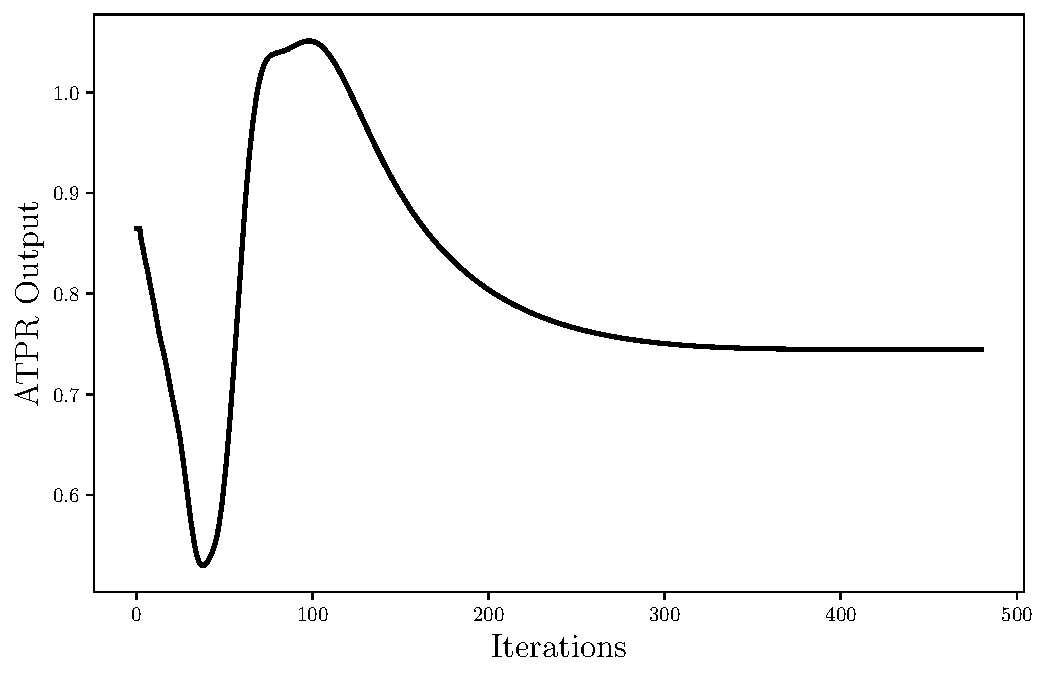
\includegraphics[width = 0.9\linewidth]{rep/q3/ATPR.pdf}
    \caption[ATPR Output for Baseline Mesh]{ATPR output for baseline mesh.}
    \label{fig:ATPR_mesh0}
\end{figure}

Next, was to check and confirm that the solution is giving a physical answer returning an ATPR that is less than one at the exit of the engine. The reason for the less than one is due to the fact that shocks are forming at the inlet of the engine resulting in a loss of total pressure due to entropy that cannot be recovered. Using Equation \ref{eqn:ATPR}, with the approximated state values I get Figure \ref{fig:ATPR_mesh0} above confirming that the solution is converging to a value that physically makes sense.

\pagebreak
\subsubsection{Baseline Field Plots}

\begin{figure}[h]
    \centering
    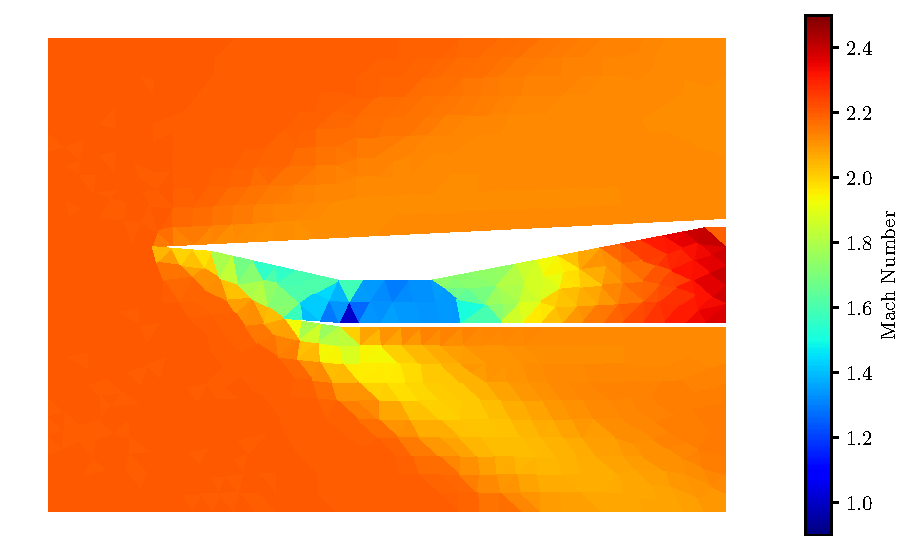
\includegraphics[width = 0.9\linewidth]{rep/q3/Machfield.pdf}
    \caption[Field Plot of Mach Number for Baseline Mesh]{Field plot of Mach number with $\alpha = 1\degree$.}
    \label{fig:mach_mesh0}
\end{figure}

\paragraph{Field Plot of Mach Number} Above in Figure \ref{fig:mach_mesh0}, is the field plot of the mach number at $M_\infty = 2.2$ at an angle of $\alpha=1\degree$. This plot shows the free-stream mach number at the steady-state with visible oblique shocks at the inlet of the engine. However, due to the coarseness of the mesh, much information is lost within the interior of the engine resulting from the train of shocks inside the inlet of the engine. The next section aims to refine this mesh to return a more refined result.

\pagebreak
\begin{figure}[h]
    \centering
    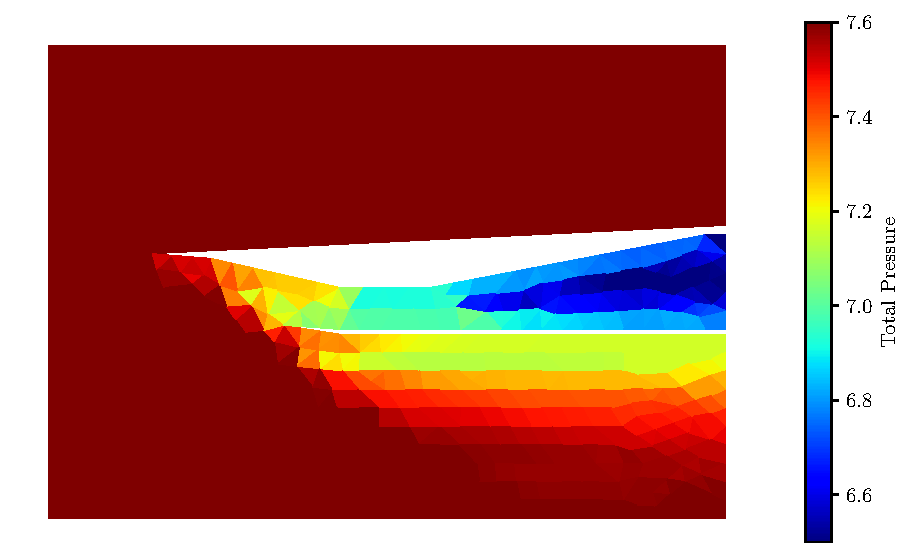
\includegraphics[width = 0.9\linewidth]{rep/q3/Pfield.pdf}
    \caption[Field Plot of Total Pressure for Baseline Mesh]{Field plot of total pressure with $\alpha = 1\degree$.}
    \label{fig:pt_mesh0}
\end{figure}

\paragraph{Field Plot of Total Pressure} Above in Figure \ref{fig:pt_mesh0}, is the field plot of the total pressure at $M_\infty$ at an angle of $\alpha=1\degree$. Similar to Figure \ref{fig:mach_mesh0}, there are some visible oblique shocks at the inlet of the engine. But similar to the mach field plot, much of the information is lost within the interior of the engine requiring more refinement of the mesh to return a more accurate solution. What can be found is that the total pressure decreases throughout the inlet of the engine which is consistent with theory through the losses associated with the shocks.